\documentclass[tikz,border=5pt]{standalone}
\usepackage{graphicx}
\usepackage{xcolor}
\usetikzlibrary{arrows.meta,calc,positioning}

\definecolor{goliatblue}{RGB}{65,91,105}
\definecolor{landmark}{RGB}{165,68,45}

\begin{document}
\begin{tikzpicture}[
  font=\rmfamily\small,
  panel/.style={draw=black, rectangle, line width=0.8pt},
  labelbox/.style={draw=black, fill=white, rectangle, align=left, inner sep=3pt,
                   font=\rmfamily\footnotesize},
  flow/.style={-{Latex[length=2.2mm]}, line width=0.7pt},
  measure/.style={<->, densely dashed, line width=0.65pt, color=goliatblue},
  landmarkline/.style={line width=0.55pt, color=landmark},
  censor/.style={draw=goliatblue!85, fill=goliatblue!42, rounded corners=0.6pt,
                 line width=0.45pt}
]
  % Near-field panel
  \draw[panel] (0,0) rectangle (8.8,6.5);
  \node[font=\rmfamily\bfseries] at (4.4,6.12) {Near-field device exposure};

  \node[inner sep=0pt] (child) at (2.45,2.95)
    {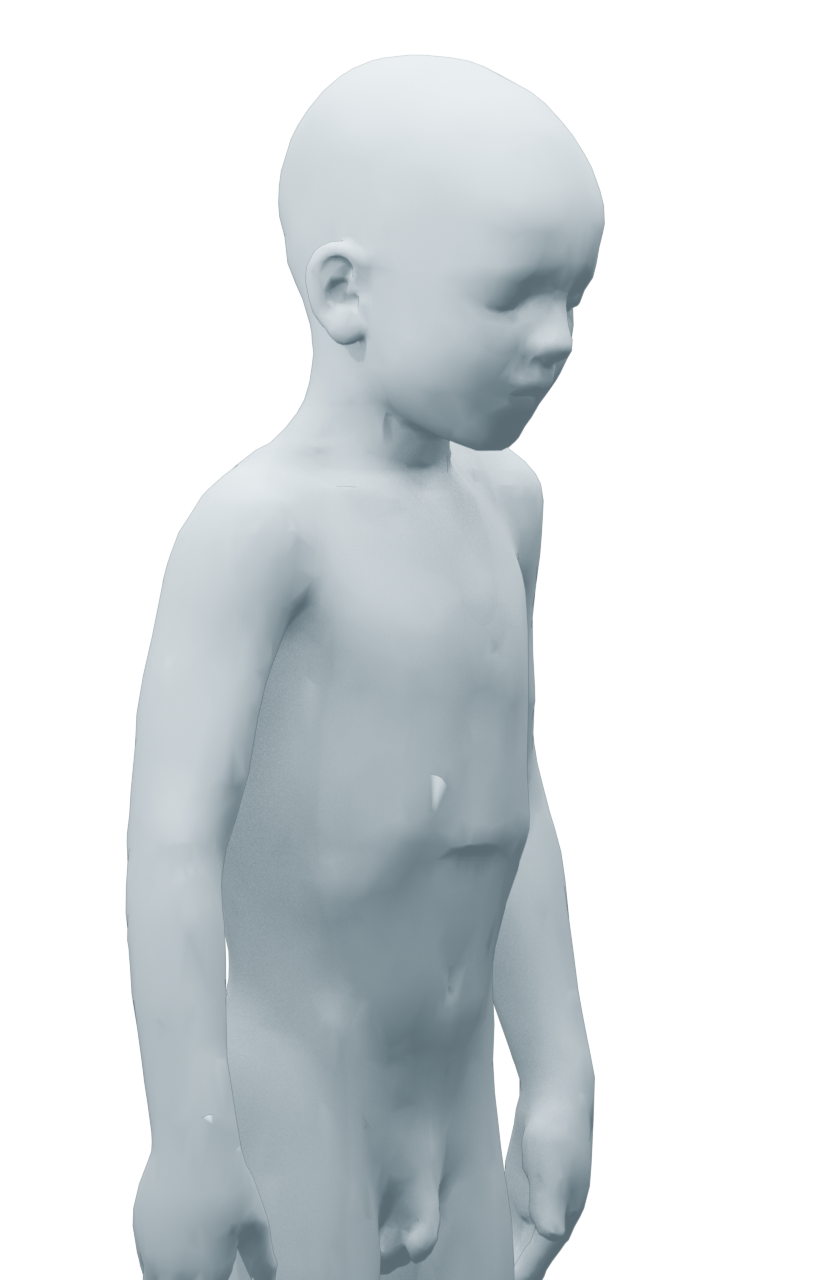
\includegraphics[height=5.20cm]{phantom_renders/thelonious_landmarks.png}};
  \draw[censor] (2.28,0.40) rectangle (2.88,0.92);
  \node[font=\rmfamily\scriptsize, text=goliatblue] at (2.45,0.18)
    {Thelonious child model};

  % Landmark positions on the closer three-quarter view.
  \fill[landmark] (3.12,4.30) circle (1.8pt);
  \draw[landmarkline] (3.12,4.30) -- (3.55,4.90);
  \node[font=\rmfamily\scriptsize, anchor=west, text=landmark] at (3.59,4.92) {Nasion};

  \fill[landmark] (2.30,4.31) circle (1.8pt);
  \draw[landmarkline] (2.30,4.31) -- (1.85,5.05);
  \node[font=\rmfamily\scriptsize, anchor=east, text=landmark] at (1.81,5.07) {Tragus};

  \fill[landmark] (2.73,2.17) circle (1.8pt);
  \draw[landmarkline] (2.73,2.17) -- (3.68,2.04);
  \node[font=\rmfamily\scriptsize, anchor=west, text=landmark] at (3.72,2.04) {Umbilicus};

  % A device is positioned from the tragus with an explicit offset.
  \draw[fill=goliatblue!30, draw=goliatblue, rounded corners=0.6pt, line width=0.8pt]
    (0.60,3.80) rectangle (0.96,4.78);
  \draw[measure] (0.98,4.31) -- (2.26,4.31);
  \node[font=\rmfamily\footnotesize, text=black, anchor=north] at (1.62,4.20) {Offset};

  \node[labelbox, text width=3.0cm, anchor=north west] at (5.00,5.33) {
    Device model and power\\
    Placement landmark\\
    Offset and orientation};
  \node[font=\rmfamily\footnotesize, align=center] at (5.93,1.00)
    {SAR or APD\\normalized to input power};

  % Far-field panel
  \draw[panel] (9.4,0) rectangle (18.2,6.5);
  \node[font=\rmfamily\bfseries] at (13.8,6.12) {Far-field environmental exposure};

  \draw[line width=0.65pt, color=goliatblue] (11.02,0.66) rectangle (14.46,5.48);
  \node[inner sep=0pt] (adult) at (12.74,3.03)
    {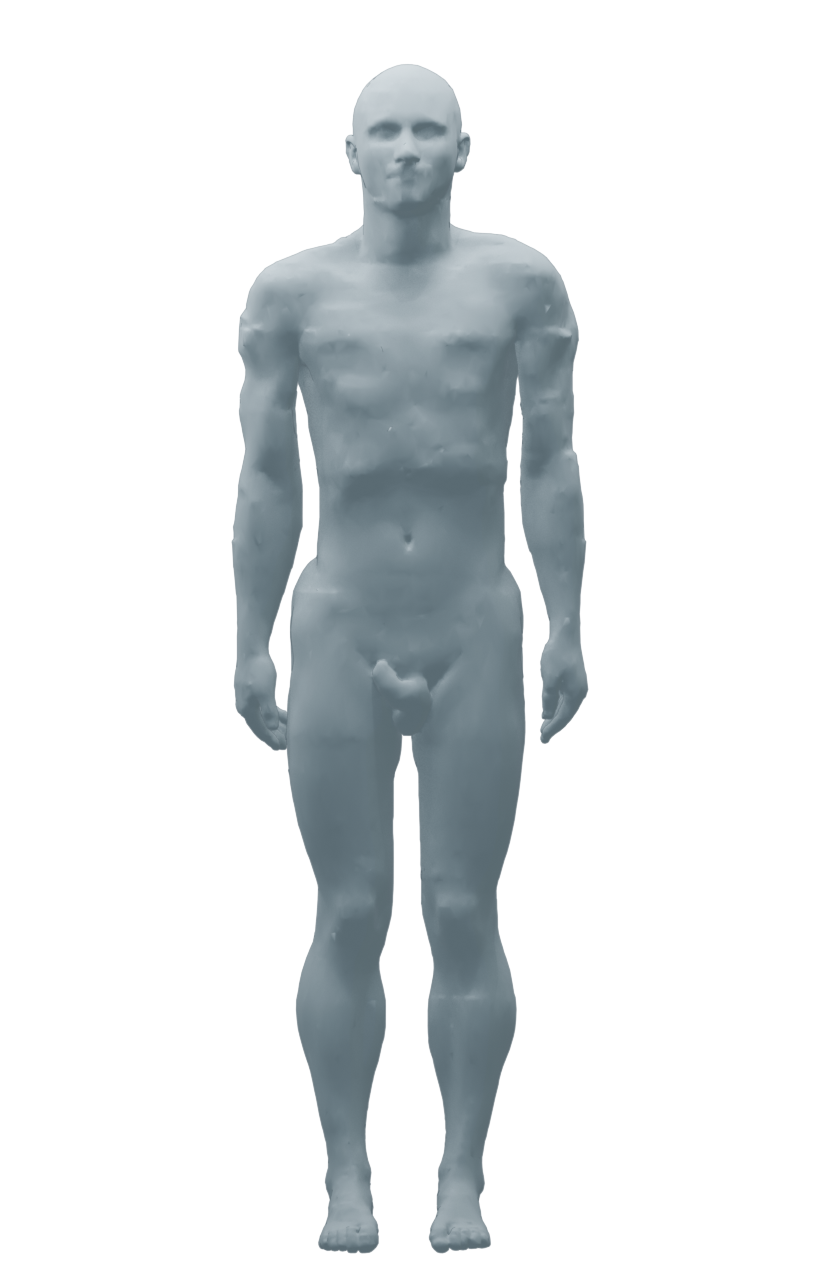
\includegraphics[height=4.65cm]{phantom_renders/duke_far_field.png}};
  \draw[censor] (12.50,2.55) rectangle (13.02,3.08);
  \node[font=\rmfamily\scriptsize, text=goliatblue] at (12.74,0.35)
    {Duke adult model};

  \foreach \y in {1.55,2.70,3.85,5.00} {
    \draw[flow, color=goliatblue] (9.62,\y) -- (10.92,\y);
  }
  \node[labelbox, text width=2.45cm, anchor=north west] at (15.05,5.32) {
    Frequency\\
    Direction\\
    Polarization\\
    Grid and domain};
  \draw[flow, densely dashed, color=goliatblue] (15.05,3.72) -- (14.48,3.72);
  \node[font=\rmfamily\footnotesize, align=center] at (16.30,1.00)
    {SAR or APD normalized to\\incident power density};

  % Shared output
  \node[labelbox, align=center, text width=7.7cm] (record) at (9.1,-1.35) {
    Shared job record: expanded JSON, phase log, and solver files\\
    Extracted results and analysis tables};
  \coordinate (recordleft) at ($(record.north west)!0.30!(record.north east)$);
  \coordinate (recordright) at ($(record.north west)!0.70!(record.north east)$);
  \draw[flow] (4.4,0) -- (4.4,-0.42) -| (recordleft);
  \draw[flow] (13.8,0) -- (13.8,-0.42) -| (recordright);
\end{tikzpicture}
\end{document}
